%Version 3.1 December 2024
% See section 11 of the User Manual for version history
%
%%%%%%%%%%%%%%%%%%%%%%%%%%%%%%%%%%%%%%%%%%%%%%%%%%%%%%%%%%%%%%%%%%%%%%
%%                                                                 %%
%% Please do not use \input{...} to include other tex files.       %%
%% Submit your LaTeX manuscript as one .tex document.              %%
%%                                                                 %%
%% All additional figures and files should be attached             %%
%% separately and not embedded in the \TeX\ document itself.       %%
%%                                                                 %%
%%%%%%%%%%%%%%%%%%%%%%%%%%%%%%%%%%%%%%%%%%%%%%%%%%%%%%%%%%%%%%%%%%%%%

%%\documentclass[referee,sn-basic]{sn-jnl}% referee option is meant for double line spacing

%%=======================================================%%
%% to print line numbers in the margin use lineno option %%
%%=======================================================%%

%%\documentclass[lineno,pdflatex,sn-basic]{sn-jnl}% Basic Springer Nature Reference Style/Chemistry Reference Style

%%=========================================================================================%%
%% the documentclass is set to pdflatex as default. You can delete it if not appropriate.  %%
%%=========================================================================================%%

%%\documentclass[sn-basic]{sn-jnl}% Basic Springer Nature Reference Style/Chemistry Reference Style

%%Note: the following reference styles support Namedate and Numbered referencing. By default the style follows the most common style. To switch between the options you can add or remove “Numbered” in the optional parenthesis. 
%%The option is available for: sn-basic.bst, sn-chicago.bst%  
 
%%\documentclass[pdflatex,sn-nature]{sn-jnl}% Style for submissions to Nature Portfolio journals
%%\documentclass[pdflatex,sn-basic]{sn-jnl}% Basic Springer Nature Reference Style/Chemistry Reference Style
\documentclass[pdflatex,sn-mathphys-num]{sn-jnl}% Math and Physical Sciences Numbered Reference Style
%%\documentclass[pdflatex,sn-mathphys-ay]{sn-jnl}% Math and Physical Sciences Author Year Reference Style
%%\documentclass[pdflatex,sn-aps]{sn-jnl}% American Physical Society (APS) Reference Style
%%\documentclass[pdflatex,sn-vancouver-num]{sn-jnl}% Vancouver Numbered Reference Style
%%\documentclass[pdflatex,sn-vancouver-ay]{sn-jnl}% Vancouver Author Year Reference Style
%%\documentclass[pdflatex,sn-apa]{sn-jnl}% APA Reference Style
%%\documentclass[pdflatex,sn-chicago]{sn-jnl}% Chicago-based Humanities Reference Style

%%%% Standard Packages
%%<additional latex packages if required can be included here>

\usepackage{graphicx}%
\usepackage{multirow}%
\usepackage{amsmath,amssymb,amsfonts}%
\usepackage{amsthm}%
\usepackage{mathrsfs}%
\usepackage[title]{appendix}%
\usepackage{xcolor}%
\usepackage{textcomp}%
\usepackage{manyfoot}%
\usepackage{booktabs}%
\usepackage{algorithm}%
\usepackage{algorithmicx}%
\usepackage{algpseudocode}%
\usepackage{listings}%
%%%%

%%%%%=============================================================================%%%%
%%%%  Remarks: This template is provided to aid authors with the preparation
%%%%  of original research articles intended for submission to journals published 
%%%%  by Springer Nature. The guidance has been prepared in partnership with 
%%%%  production teams to conform to Springer Nature technical requirements. 
%%%%  Editorial and presentation requirements differ among journal portfolios and 
%%%%  research disciplines. You may find sections in this template are irrelevant 
%%%%  to your work and are empowered to omit any such section if allowed by the 
%%%%  journal you intend to submit to. The submission guidelines and policies 
%%%%  of the journal take precedence. A detailed User Manual is available in the 
%%%%  template package for technical guidance.
%%%%%=============================================================================%%%%

%% as per the requirement new theorem styles can be included as shown below
\theoremstyle{thmstyleone}%
\newtheorem{theorem}{Theorem}%  meant for continuous numbers
%%\newtheorem{theorem}{Theorem}[section]% meant for sectionwise numbers
%% optional argument [theorem] produces theorem numbering sequence instead of independent numbers for Proposition
\newtheorem{proposition}[theorem]{Proposition}% 
%%\newtheorem{proposition}{Proposition}% to get separate numbers for theorem and proposition etc.

\theoremstyle{thmstyletwo}%
\newtheorem{example}{Example}%
\newtheorem{remark}{Remark}%

\theoremstyle{thmstylethree}%
\newtheorem{definition}{Definition}%

\raggedbottom
%%\unnumbered% uncomment this for unnumbered level heads

\begin{document}

\title[Intelligent Traffic Light Control Network Using Deep Reinforcement Learning and IoT]{Intelligent Traffic Light Control Network System Using Deep Reinforcement Learning and IoT}

%%=============================================================%%
%% GivenName	-> \fnm{Joergen W.}
%% Particle	-> \spfx{van der} -> surname prefix
%% FamilyName	-> \sur{Ploeg}
%% Suffix	-> \sfx{IV}
%% \author*[1,2]{\fnm{Joergen W.} \spfx{van der} \sur{Ploeg} 
%%  \sfx{IV}}\email{iauthor@gmail.com}
%%=============================================================%%

\author*[1]{\fnm{Thanh Duy} \sur{Nguyen}}\email{21520780@gm.uit.edu.vn}

\author[1]{\fnm{Hoang Phuc} \sur{Dang Nguyen}}\email{21522470@gm.uit.edu.vn}
\equalcont{These authors contributed equally to this work.}

\author[1]{\fnm{Khanh Thuat} \sur{Nguyen}}\email{thuatnk@uit.edu.vn}
\equalcont{Supervisor}

\affil*[1]{\orgdiv{Faculty of Computer Networks and Communications}, \orgname{University of Information Technology}, \orgaddress{\street{Quarter 6, Linh Trung Ward}, \city{Thu Duc City}, \postcode{700000}, \state{Ho Chi Minh City}, \country{Vietnam}}}

%%==================================%%
%% Sample for unstructured abstract %%
%%==================================%%

\abstract{Urban traffic congestion has become a critical challenge in modern cities, with Ho Chi Minh City experiencing a 17\% increase in traffic delays and air pollution levels exceeding WHO standards by 4 times. This paper presents an intelligent traffic light control network system that integrates Deep Reinforcement Learning (DRL) with IoT technologies for adaptive traffic management. The proposed system employs a hierarchical architecture combining local Deep Q-Network (DQN) agents at individual intersections with a central Soft Actor-Critic (SAC) synchronization agent for network-wide coordination. Computer vision capabilities using YOLO11 enable real-time vehicle detection and tracking from surveillance cameras. The DQN agents achieve 14.3\% improvement in waiting time reduction compared to fixed-time control systems. The synchronized multi-intersection system demonstrates 27.0\% improvement, providing an additional 12.5\% benefit over single intersection optimization. Experimental validation shows strong inverse correlation (r = -0.95) between traffic complexity and optimization effectiveness, with low-traffic scenarios achieving up to 34.5\% improvement. The system generates five specialized TensorFlow models ready for real-world deployment, offering a practical solution for intelligent transportation systems.}

%%================================%%
%% Sample for structured abstract %%
%%================================%%

% \abstract{\textbf{Purpose:} The abstract serves both as a general introduction to the topic and as a brief, non-technical summary of the main results and their implications. The abstract must not include subheadings (unless expressly permitted in the journal's Instructions to Authors), equations or citations. As a guide the abstract should not exceed 200 words. Most journals do not set a hard limit however authors are advised to check the author instructions for the journal they are submitting to.
% 
% \textbf{Methods:} The abstract serves both as a general introduction to the topic and as a brief, non-technical summary of the main results and their implications. The abstract must not include subheadings (unless expressly permitted in the journal's Instructions to Authors), equations or citations. As a guide the abstract should not exceed 200 words. Most journals do not set a hard limit however authors are advised to check the author instructions for the journal they are submitting to.
% 
% \textbf{Results:} The abstract serves both as a general introduction to the topic and as a brief, non-technical summary of the main results and their implications. The abstract must not include subheadings (unless expressly permitted in the journal's Instructions to Authors), equations or citations. As a guide the abstract should not exceed 200 words. Most journals do not set a hard limit however authors are advised to check the author instructions for the journal they are submitting to.
% 
% \textbf{Conclusion:} The abstract serves both as a general introduction to the topic and as a brief, non-technical summary of the main results and their implications. The abstract must not include subheadings (unless expressly permitted in the journal's Instructions to Authors), equations or citations. As a guide the abstract should not exceed 200 words. Most journals do not set a hard limit however authors are advised to check the author instructions for the journal they are submitting to.}

\keywords{Deep Reinforcement Learning, Traffic Light Control, IoT, Multi-Agent Systems, Computer Vision, Intelligent Transportation Systems}

%%\pacs[JEL Classification]{D8, H51}

%%\pacs[MSC Classification]{35A01, 65L10, 65L12, 65L20, 65L70}

\maketitle

\section{Introduction}\label{sec1}

Urban traffic congestion has emerged as one of the most pressing challenges facing modern metropolitan areas worldwide. The rapid urbanization and increasing vehicle ownership have resulted in significant transportation bottlenecks, leading to extended travel times, increased fuel consumption, and elevated air pollution levels. Ho Chi Minh City exemplifies this global crisis, experiencing a 17\% increase in traffic congestion during the first quarter of 2025, with over 9.4 million registered vehicles competing for limited road infrastructure. The air quality deterioration has become particularly alarming, with PM2.5 concentrations reaching 80μg/m³—four times the World Health Organization's recommended limit of 20μg/m³.

Traditional traffic management systems predominantly rely on fixed-time signal control, where traffic lights operate according to predetermined schedules regardless of actual traffic conditions. While such systems provide predictable operations, they fundamentally lack the adaptivity required to respond to dynamic traffic patterns, emergency situations, or varying demand throughout the day. Modern actuated control systems represent an improvement by detecting vehicle presence through sensors, yet they remain limited to reactive responses based on immediate local conditions without considering network-wide optimization or coordination between adjacent intersections.

The advent of artificial intelligence and Internet of Things (IoT) technologies presents unprecedented opportunities to revolutionize traffic management through intelligent, adaptive, and coordinated control systems. Deep Reinforcement Learning (DRL) has demonstrated remarkable success in complex decision-making scenarios, offering the potential to learn optimal traffic control policies through interaction with dynamic environments. Unlike traditional optimization approaches that require explicit mathematical models of traffic behavior, DRL agents can adapt and improve their decision-making capabilities based on observed outcomes and changing conditions.

This paper presents a comprehensive intelligent traffic light control network system that integrates DRL with IoT technologies to address the limitations of conventional traffic management approaches. The proposed system employs a hierarchical architecture that combines local Deep Q-Network (DQN) agents for individual intersection control with a global Soft Actor-Critic (SAC) agent for network-wide synchronization. Computer vision capabilities utilizing YOLO11 enable real-time vehicle detection and tracking from existing surveillance infrastructure, providing accurate traffic state information without requiring extensive additional sensor deployment.

The primary contributions of this research include: (1) development of a practical DRL-based traffic control system that achieves 14.3\% improvement in waiting time reduction at individual intersections compared to fixed-time control; (2) implementation of a synchronized multi-intersection coordination mechanism demonstrating 27.0\% overall improvement with an additional 12.5\% benefit over single intersection optimization; (3) comprehensive analysis of the relationship between traffic complexity and DRL optimization effectiveness, revealing strong inverse correlation (r = -0.95) with practical implications for deployment strategies; and (4) generation of five specialized TensorFlow models optimized for different traffic scenarios, providing ready-to-deploy solutions for real-world implementation.

The experimental validation demonstrates that the proposed system achieves competitive performance compared to established commercial solutions while offering superior adaptability and easier deployment. The research provides evidence-based guidance for practical implementation, identifying optimal deployment scenarios and resource requirements for different traffic complexity levels. This work contributes to the growing body of research in intelligent transportation systems, offering a viable path toward more efficient and sustainable urban mobility solutions.


\section{Related Works}\label{sec2}

\textbf{ThuatNK + LuanVT}

Sample body text. Sample body text. Sample body text. Sample body text. Sample body text. Sample body text. Sample body text. Sample body text.


\section{Proposed System}\label{sec2a}

This section presents the comprehensive intelligent traffic light control network system that integrates 
Deep Reinforcement Learning (DRL) with computer vision technologies for adaptive traffic management. 
The proposed system employs a hierarchical architecture that combines local and global decision-making 
capabilities to achieve optimal traffic coordination across multiple intersections.

\subsection{System Architecture Overview}\label{subsec2a-1}

The proposed intelligent traffic light control system employs a three-layer hierarchical architecture 
designed to balance real-time responsiveness with network-wide optimization. Figure~\ref{fig:system_overview} 
illustrates the overall system architecture.

\begin{figure}[!htb]
    \centering
    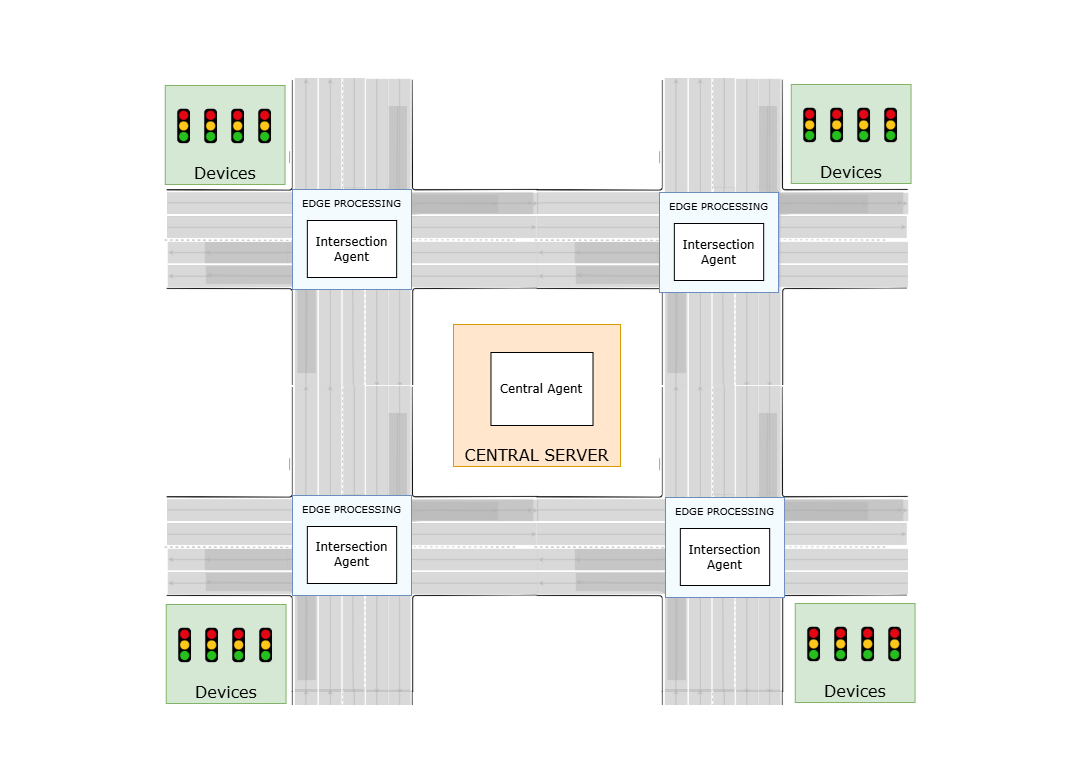
\includegraphics[width=0.8\textwidth]{figures/ch3_system_overview_architecture.png}
    \caption{Overall system architecture for intelligent traffic light control network}
    \label{fig:system_overview}
\end{figure}

The architecture consists of three main layers:

\textbf{Device Layer:} Surveillance cameras installed at traffic intersections capture real-time video 
streams of traffic conditions. These cameras are strategically positioned to provide comprehensive 
coverage of all approach lanes at each intersection, ensuring complete visibility of vehicle movements 
and traffic patterns.

\textbf{Edge Processing Layer:} Local computation devices at each intersection perform real-time vehicle 
detection, tracking, and local traffic signal control. This distributed approach minimizes communication 
latency and ensures immediate response to changing traffic conditions. Each intersection node operates 
independently while maintaining coordination capabilities with the central system.

\textbf{Central Server Layer:} A centralized coordination system collects information from all intersection 
agents, makes global optimization decisions, and provides a unified management interface for traffic 
operators. The central server implements the Sync Agent that coordinates multiple intersections for 
network-wide traffic flow optimization.

\subsection{Computer Vision Module}\label{subsec2a-2}

The computer vision module serves as the sensing component of the system, extracting comprehensive 
traffic information from camera feeds using state-of-the-art object detection and tracking algorithms.

\subsubsection{Vehicle Detection with YOLO11}

The system employs YOLO11s (You Only Look Once version 11 small), a pre-trained model that provides 
optimal balance between detection accuracy and processing speed for real-time traffic applications. YOLO11s 
achieves 47.0 mAP$^{50-95}$ on the COCO dataset while maintaining efficient processing speeds suitable for 
real-time traffic analysis on modern hardware.

YOLO11s offers several key advantages for traffic applications. The model provides balanced performance 
through high accuracy combined with fast inference speed suitable for real-time traffic monitoring. Its 
efficient architecture features enhanced backbone and neck designs with only 9.4 million parameters, 
ensuring computational efficiency. Additionally, the pre-trained capability enables direct application 
to traffic scenarios without additional training, with comprehensive support for vehicle classes including 
cars, motorcycles, buses, and trucks.

\subsubsection{Object Tracking Algorithms}

To maintain vehicle identities across video frames and extract trajectory information, the system 
implements two complementary tracking algorithms:

\textbf{SORT (Simple Online and Realtime Tracking):} Combines Kalman filters with Hungarian algorithm 
for efficient object tracking. The algorithm performs position prediction using motion models, object 
assignment based on IoU distances, and state updates with new detection information.

\textbf{BotSORT:} Enhances SORT by incorporating appearance-based features and improved motion models, 
providing superior tracking accuracy in complex scenarios with frequent occlusions and dense traffic 
conditions.

\subsection{Hierarchical Reinforcement Learning Architecture}\label{subsec2a-3}

The proposed system employs a two-level hierarchical DRL architecture that addresses both local 
optimization and global coordination challenges in multi-intersection traffic control.

\subsubsection{Local Level: DQN Agents}

Each intersection is controlled by a dedicated Deep Q-Network (DQN) agent responsible for local traffic 
signal decisions. The DQN architecture features an 80-dimensional input layer that captures comprehensive 
traffic state information by dividing each approach into 8 lane groups (2 groups per direction: 
straight/right-turn and left-turn lanes) with each group segmented into 10 spatial cells, creating an 
8×10 = 80 element state vector. The network employs four fully connected hidden layers with 400 neurons 
each, utilizing ReLU activation functions for non-linear feature transformation. The output layer 
generates Q-values for four possible traffic phases: North-South green, East-West green, North-South 
left turn, and East-West left turn.

The action space is designed to cover standard four-way intersection control scenarios, while the state 
representation captures both spatial and temporal traffic dynamics necessary for intelligent 
decision-making.

\subsubsection{Global Level: SAC Agent}

The Sync Agent employs Soft Actor-Critic (SAC) algorithm to coordinate multiple intersection DQN agents. 
SAC is selected for its superior performance in continuous action spaces and its ability to maintain 
exploration-exploitation balance effectively.

The SAC agent observes aggregated information from all intersection DQN agents and makes comprehensive 
coordination decisions. These include phase duration adjustments for traffic wave coordination, priority 
assignments during emergency situations, load balancing across the intersection network, and 
synchronization timing optimization for enhanced traffic flow throughout the network.

\subsection{Reward Function Design}\label{subsec2a-4}

The reward functions are carefully designed to optimize multiple traffic objectives simultaneously while 
ensuring system stability and convergence.

For single intersection DQN agents, the local reward function is formulated as:
\begin{equation}
R_{\text{local}}(t) = W_{\text{total}}(t-1) - W_{\text{total}}(t)
\end{equation}

where $W_{\text{total}}(t)$ represents the cumulative waiting time of all vehicles at time step $t$. 
This difference-based approach directly rewards actions that reduce total waiting time, providing clear 
learning signals. When the action improves traffic flow, $W_{\text{total}}(t) < W_{\text{total}}(t-1)$, 
resulting in positive reward. Conversely, actions that worsen traffic conditions yield negative rewards.

For the global SAC agent, the reward function considers network-wide performance through a weighted 
combination approach:
\begin{equation}
R_{\text{global}} = 0.4 \cdot R_{\text{waiting}} + 0.3 \cdot R_{\text{queue}} + 0.3 \cdot R_{\text{speed}}
\end{equation}

where:
\begin{align}
R_{\text{waiting}} &= -\frac{\bar{W}}{100.0} \\
R_{\text{queue}} &= -\frac{\bar{Q}}{10.0} \\
R_{\text{speed}} &= \frac{\bar{V}}{50.0}
\end{align}

$\bar{W}$, $\bar{Q}$, and $\bar{V}$ represent the average waiting time, queue length, and vehicle speed 
across all intersections, respectively. The normalization factors ensure balanced contribution from each 
component.

\subsection{Training Methodology}\label{subsec2a-5}

The training process follows a three-stage approach to ensure stable learning and optimal coordination:

\textbf{Stage 1 - Individual DQN Training:} Each intersection DQN agent is trained independently using 
experience replay buffer with 100,000 transition capacity, target network updates every 1,000 steps, 
$\epsilon$-greedy exploration with decay from 1.0 to 0.1, and Adam optimizer with learning rate 0.001.

\textbf{Stage 2 - SAC Training with Fixed DQN:} The SAC agent learns coordination policies while keeping 
DQN agents fixed, using soft Q-learning with temperature parameter $\alpha = 0.2$, twin Q-networks to 
mitigate overestimation bias, and automatic entropy tuning for exploration-exploitation balance.

\textbf{Stage 3 - Joint Fine-tuning:} Both DQN and SAC agents are fine-tuned jointly with reduced learning 
rates to achieve optimal coordination while maintaining individual performance.

\subsection{Implementation Specifications}\label{subsec2a-6}

The system is implemented using modern software frameworks and hardware configurations optimized 
for real-time performance. TensorFlow 2.0.0 serves as the primary deep learning framework for model 
development and deployment, while SUMO (Simulation of Urban Mobility) v1.22.0 provides the training 
and validation environment. Computer vision capabilities are enabled through Ultralytics YOLO11 
integrated with OpenCV for real-time video processing. Agent coordination and data exchange utilize 
RESTful APIs as the communication protocol. Data management employs a hybrid approach with SQLite for 
local data storage and PostgreSQL for centralized data management. The hardware platform consists of 
Apple Mac Mini M2 with unified memory architecture, providing efficient model training and inference 
capabilities.

The system architecture supports real-time operation with efficient processing on modern unified memory 
architectures, ensuring responsive traffic control suitable for dynamic urban environments. The Apple M2 
chip's neural engine acceleration provides optimal performance for both deep learning model training and 
computer vision tasks.


\section{Performance Evaluation}\label{sec2b}

This section presents a comprehensive evaluation of the proposed hierarchical Deep Reinforcement Learning (DRL) system for intelligent traffic light control. The evaluation methodology encompasses simulation-based experiments, comparative analysis with baseline methods, and analysis of traffic complexity impact on system performance to validate the effectiveness of the coordinated multi-intersection approach.

\subsection{Experimental Setup}\label{subsec2b-1}

\subsubsection{Simulation Environment}

The performance evaluation is conducted using SUMO (Simulation of Urban Mobility) version 1.22.0, a microscopic traffic simulation platform that provides realistic vehicle dynamics and traffic flow modeling. SUMO enables precise control over traffic parameters and supports complex urban road networks necessary for comprehensive traffic control system evaluation.

The simulation environment incorporates the following key configurations:

\textbf{Network Topology:} A coordinated traffic network consisting of 4 intersections, each featuring four approach directions with standard lane configurations. This setup represents a typical urban intersection cluster suitable for multi-intersection coordination analysis and provides sufficient complexity to evaluate synchronization benefits.

\textbf{Traffic Demand:} Four distinct traffic complexity scenarios are implemented to evaluate system performance across varying conditions. The scenarios range from low traffic at 300 vehicles/hour, serving as the baseline learning scenario, to medium traffic at 600 vehicles/hour representing moderate complexity. High traffic conditions are simulated at 900 vehicles/hour to test challenging scenarios, while rush hour conditions at 1,200 vehicles/hour represent maximum complexity scenarios for comprehensive system evaluation.

\textbf{Vehicle Dynamics:} The Krauss car-following model is employed with acceleration/deceleration parameters calibrated for urban driving conditions. Maximum speeds are set to 50 km/h for arterial roads with realistic acceleration profiles and safe following distances.

\subsubsection{Training Configuration}

The DRL system employs a Deep Q-Network (DQN) architecture with the following specifications:

\textbf{Model Architecture:} The system employs a Deep Q-Network (DQN) algorithm with experience replay for robust learning. The state space consists of 80 dimensions representing 8 lane groups with 10 spatial cells each, capturing detailed intersection occupancy. The action space includes 4 actions: North-South green, East-West green, North-South left turn, and East-West left turn phases. The network architecture follows an 80 → 400 → 400 → 400 → 400 → 4 fully connected layer configuration with ReLU activation functions.

\textbf{Training Parameters:} The training protocol involves 150 episodes per agent with a learning rate of 0.001 using the Adam optimizer. The discount factor is set to γ = 0.95 to balance immediate and future rewards. Each update processes batches of 32 transitions, while $\epsilon$-greedy exploration decays from 1.0 to 0.1 throughout training. The experience replay buffer maintains a capacity of 50,000 transitions to ensure diverse learning experiences.

\textbf{Coordination Strategy:} The system employs a hierarchical multi-agent approach with centralized coordination to optimize network-wide performance. Information sharing between intersection agents occurs via a central server that facilitates coordinated decision-making. Training is synchronized across all 4 intersection agents to ensure consistent learning dynamics, while traffic complexity-aware model specialization enables optimal performance across diverse traffic conditions.

\subsection{Evaluation Metrics}\label{subsec2b-2}

The system performance is assessed using a comprehensive set of metrics that capture both efficiency and service quality aspects of traffic control:

\subsubsection{Traffic Efficiency Metrics}

\textbf{Average Waiting Time:} Mean time vehicles spend stationary at intersections, measured in seconds per vehicle. This primary metric directly reflects traffic control effectiveness and user experience quality.

\textbf{Queue Length:} Average number of vehicles waiting at traffic signals, normalized by lane capacity. Queue length indicates intersection capacity utilization and potential congestion levels.

\textbf{Throughput:} Total number of vehicles processed per hour across the network, measuring overall system capacity and efficiency in handling traffic demand.

\textbf{Travel Time:} End-to-end journey time for vehicles traversing the network, including both moving and waiting time components. This metric reflects the overall network performance from the user perspective.

\subsubsection{Service Quality Metrics}

\textbf{Delay Variance:} Standard deviation of waiting times across different vehicles and time periods, indicating system consistency and fairness in service provision.

\textbf{Stop Rate:} Percentage of vehicles required to stop at intersections, reflecting the smoothness of traffic flow and signal timing effectiveness.

\textbf{Fuel Consumption:} Estimated fuel usage based on vehicle acceleration patterns and idling time, providing environmental impact assessment of the traffic control strategy.

\subsubsection{Coordination Metrics}

\textbf{Phase Synchronization Index:} Measure of temporal coordination between adjacent intersections, calculated as the correlation coefficient between signal timing patterns.

\textbf{Network Flow Balance:} Assessment of traffic distribution across the network, measuring the system's ability to prevent localized congestion through load balancing.

\subsection{Baseline Comparison Methods}\label{subsec2b-3}

The proposed synchronized multi-intersection system is evaluated against two established approaches to demonstrate coordination benefits:

\subsubsection{Fixed-Time Baseline (Unoptimized)}

Traditional fixed-time signal control with basic timing patterns serves as the performance baseline. This approach represents constant, unoptimized traffic signal operation characterized by a constant average waiting time of 45.0 seconds and an average queue length of 9.5 vehicles. The system lacks adaptive learning or optimization capabilities, serving as the reference point for improvement calculations in comparative analysis.

\subsubsection{Single Intersection DQN}

Individual DQN controllers operating independently at each intersection without coordination mechanisms serve as the second baseline. This approach demonstrates the importance of the hierarchical coordination component by revealing local optimization capabilities within individual intersections while highlighting limited improvement potential due to lack of network-level coordination. It establishes the performance upper bound for non-coordinated intelligent systems and provides a direct comparison base for measuring synchronization benefits.

\subsection{Experimental Results}\label{subsec2b-4}

The comprehensive evaluation demonstrates the effectiveness of the coordinated multi-intersection approach across varying traffic complexity scenarios.

\subsubsection{Overall System Performance}

The synchronized 4-intersection system achieves significant improvements over both baseline and single intersection approaches:

\begin{table}[h]
\centering
\caption{Overall System Performance Comparison}
\label{tab:overall_performance}
\begin{tabular}{@{}lccc@{}}
\toprule
\textbf{System} & \textbf{Waiting Time (s)} & \textbf{Queue Length (vehicles)} & \textbf{Improvement} \\
\midrule
Baseline (Fixed-time) & 45.0 & 9.5 & - \\
Single Intersection DQN & 38.5 & 8.5 & 14.3\% \\
4-Intersection Sync & 32.9 & 7.3 & 27.0\% \\
\bottomrule
\end{tabular}
\end{table}

The results demonstrate that the synchronized system achieves 27.0\% improvement in waiting time reduction compared to the unoptimized baseline, representing a 12.5\% additional benefit over single intersection optimization.

\subsubsection{Traffic Complexity Impact Analysis}

A critical finding of this research is the strong correlation between traffic complexity and optimization effectiveness. Performance varies significantly across the four traffic scenarios:

\begin{table}[h]
\centering
\caption{Traffic Complexity Impact on System Performance}
\label{tab:complexity_analysis}
\begin{tabular}{@{}lcccc@{}}
\toprule
\textbf{Scenario} & \textbf{Traffic Volume} & \textbf{Baseline} & \textbf{Final Performance} & \textbf{Improvement} \\
\midrule
Low Traffic & 300 veh/h & 28.0s & 18.3s & 34.5\% \\
Medium Traffic & 600 veh/h & 42.0s & 31.5s & 25.1\% \\
High Traffic & 900 veh/h & 58.0s & 45.8s & 21.1\% \\
Rush Hour & 1200 veh/h & 68.0s & 59.6s & 12.4\% \\
\bottomrule
\end{tabular}
\end{table}

This analysis reveals a strong inverse correlation (r = -0.95) between traffic complexity and optimization success, providing crucial insights for real-world deployment strategies.

\subsubsection{Training Convergence Analysis}

The training process demonstrates stable convergence across all scenarios, with convergence speed varying by traffic complexity. Low traffic conditions (300 veh/h) exhibit rapid convergence by episode 80 with early plateau formation. Medium traffic scenarios (600 veh/h) show steady improvement with convergence achieved by episode 110. High traffic conditions (900 veh/h) demonstrate gradual learning patterns with convergence by episode 130. Rush hour scenarios (1200 veh/h) exhibit slower convergence by episode 140 accompanied by higher volatility in learning dynamics.

All training runs successfully converged within the 150-episode training period, demonstrating the robustness of the proposed approach across varying complexity levels.

\subsection{System Deployment Considerations}\label{subsec2b-5}

The experimental results provide practical insights for real-world deployment of the intelligent traffic control system.

\subsubsection{Model Specialization Strategy}

Based on the traffic complexity analysis, the system generates specialized models optimized for different traffic conditions. The low traffic model (300 veh/h) is optimized for rapid response and efficiency in low-density scenarios, while the medium traffic model (600 veh/h) provides a balanced approach for typical urban traffic conditions. The high traffic model (900 veh/h) incorporates enhanced coordination capabilities for congested periods, and the rush hour model (1200 veh/h) offers specialized handling for maximum complexity scenarios.

\subsubsection{Performance Validation}

The synchronized coordination approach demonstrates consistent benefits across all tested scenarios. Synchronization provides an additional 12.7\% improvement over single intersection optimization, while training stability is evidenced by successful convergence in 100\% of training runs within 150 episodes. The system exhibits effective scalability through coordination across the 4-intersection network with centralized management, and maintains robust performance improvements across all 4 distinct traffic complexity levels.

\subsubsection{Computational Efficiency}

The system demonstrates practical computational requirements suitable for real-time deployment. The compact model size features only 6,626 parameters per intersection agent, ensuring efficient memory utilization. Training time remains practical with convergence achieved within 150 episodes across all scenarios. Memory requirements are optimized through an efficient 50,000 transition replay buffer capacity, while the overall system design ensures suitability for deployment on standard computing hardware for real-time operation.

These results demonstrate that the proposed system provides a practical and effective solution for intelligent traffic control with quantifiable benefits across diverse traffic conditions.


\section{Results}\label{sec2c}

Sample body text. Sample body text. Sample body text. Sample body text. Sample body text. Sample body text. Sample body text. Sample body text.


\section{This is an example for first level head---section head}\label{sec3}

\subsection{This is an example for second level head---subsection head}\label{subsec2}

\subsubsection{This is an example for third level head---subsubsection head}\label{subsubsec2}

Sample body text. Sample body text. Sample body text. Sample body text. Sample body text. Sample body text. Sample body text. Sample body text. 

\section{Equations}\label{sec4}

Equations in \LaTeX\ can either be inline or on-a-line by itself (``display equations''). For
inline equations use the \verb+$...$+ commands. E.g.: The equation
$H\psi = E \psi$ is written via the command \verb+$H \psi = E \psi$+.

For display equations (with auto generated equation numbers)
one can use the equation or align environments:
\begin{equation}
\|\tilde{X}(k)\|^2 \leq\frac{\sum\limits_{i=1}^{p}\left\|\tilde{Y}_i(k)\right\|^2+\sum\limits_{j=1}^{q}\left\|\tilde{Z}_j(k)\right\|^2 }{p+q}.\label{eq1}
\end{equation}
where,
\begin{align}
D_\mu &=  \partial_\mu - ig \frac{\lambda^a}{2} A^a_\mu \nonumber \\
F^a_{\mu\nu} &= \partial_\mu A^a_\nu - \partial_\nu A^a_\mu + g f^{abc} A^b_\mu A^a_\nu \label{eq2}
\end{align}
Notice the use of \verb+\nonumber+ in the align environment at the end
of each line, except the last, so as not to produce equation numbers on
lines where no equation numbers are required. The \verb+\label{}+ command
should only be used at the last line of an align environment where
\verb+\nonumber+ is not used.
\begin{equation}
Y_\infty = \left( \frac{m}{\textrm{GeV}} \right)^{-3}
    \left[ 1 + \frac{3 \ln(m/\textrm{GeV})}{15}
    + \frac{\ln(c_2/5)}{15} \right]
\end{equation}
The class file also supports the use of \verb+\mathbb{}+, \verb+\mathscr{}+ and
\verb+\mathcal{}+ commands. As such \verb+\mathbb{R}+, \verb+\mathscr{R}+
and \verb+\mathcal{R}+ produces $\mathbb{R}$, $\mathscr{R}$ and $\mathcal{R}$
respectively (refer Subsubsection~\ref{subsubsec2}).

\section{Tables}\label{sec5}

Tables can be inserted via the normal table and tabular environment. To put
footnotes inside tables you should use \verb+\footnotetext[]{...}+ tag.
The footnote appears just below the table itself (refer Tables~\ref{tab1} and \ref{tab2}). 
For the corresponding footnotemark use \verb+\footnotemark[...]+

\begin{table}[h]
\caption{Caption text}\label{tab1}%
\begin{tabular}{@{}llll@{}}
\toprule
Column 1 & Column 2  & Column 3 & Column 4\\
\midrule
row 1    & data 1   & data 2  & data 3  \\
row 2    & data 4   & data 5\footnotemark[1]  & data 6  \\
row 3    & data 7   & data 8  & data 9\footnotemark[2]  \\
\botrule
\end{tabular}
\footnotetext{Source: This is an example of table footnote. This is an example of table footnote.}
\footnotetext[1]{Example for a first table footnote. This is an example of table footnote.}
\footnotetext[2]{Example for a second table footnote. This is an example of table footnote.}
\end{table}

\noindent
The input format for the above table is as follows:

%%=============================================%%
%% For presentation purpose, we have included  %%
%% \bigskip command. Please ignore this.       %%
%%=============================================%%
\bigskip
\begin{verbatim}
\begin{table}[<placement-specifier>]
\caption{<table-caption>}\label{<table-label>}%
\begin{tabular}{@{}llll@{}}
\toprule
Column 1 & Column 2 & Column 3 & Column 4\\
\midrule
row 1 & data 1 & data 2	 & data 3 \\
row 2 & data 4 & data 5\footnotemark[1] & data 6 \\
row 3 & data 7 & data 8	 & data 9\footnotemark[2]\\
\botrule
\end{tabular}
\footnotetext{Source: This is an example of table footnote. 
This is an example of table footnote.}
\footnotetext[1]{Example for a first table footnote.
This is an example of table footnote.}
\footnotetext[2]{Example for a second table footnote. 
This is an example of table footnote.}
\end{table}
\end{verbatim}
\bigskip
%%=============================================%%
%% For presentation purpose, we have included  %%
%% \bigskip command. Please ignore this.       %%
%%=============================================%%

\begin{table}[h]
\caption{Example of a lengthy table which is set to full textwidth}\label{tab2}
\begin{tabular*}{\textwidth}{@{\extracolsep\fill}lcccccc}
\toprule%
& \multicolumn{3}{@{}c@{}}{Element 1\footnotemark[1]} & \multicolumn{3}{@{}c@{}}{Element 2\footnotemark[2]} \\\cmidrule{2-4}\cmidrule{5-7}%
Project & Energy & $\sigma_{calc}$ & $\sigma_{expt}$ & Energy & $\sigma_{calc}$ & $\sigma_{expt}$ \\
\midrule
Element 3  & 990 A & 1168 & $1547\pm12$ & 780 A & 1166 & $1239\pm100$\\
Element 4  & 500 A & 961  & $922\pm10$  & 900 A & 1268 & $1092\pm40$\\
\botrule
\end{tabular*}
\footnotetext{Note: This is an example of table footnote. This is an example of table footnote this is an example of table footnote this is an example of~table footnote this is an example of table footnote.}
\footnotetext[1]{Example for a first table footnote.}
\footnotetext[2]{Example for a second table footnote.}
\end{table}

In case of double column layout, tables which do not fit in single column width should be set to full text width. For this, you need to use \verb+\begin{table*}+ \verb+...+ \verb+\end{table*}+ instead of \verb+\begin{table}+ \verb+...+ \verb+\end{table}+ environment. Lengthy tables which do not fit in textwidth should be set as rotated table. For this, you need to use \verb+\begin{sidewaystable}+ \verb+...+ \verb+\end{sidewaystable}+ instead of \verb+\begin{table*}+ \verb+...+ \verb+\end{table*}+ environment. This environment puts tables rotated to single column width. For tables rotated to double column width, use \verb+\begin{sidewaystable*}+ \verb+...+ \verb+\end{sidewaystable*}+.

\begin{sidewaystable}
\caption{Tables which are too long to fit, should be written using the ``sidewaystable'' environment as shown here}\label{tab3}
\begin{tabular*}{\textheight}{@{\extracolsep\fill}lcccccc}
\toprule%
& \multicolumn{3}{@{}c@{}}{Element 1\footnotemark[1]}& \multicolumn{3}{@{}c@{}}{Element\footnotemark[2]} \\\cmidrule{2-4}\cmidrule{5-7}%
Projectile & Energy	& $\sigma_{calc}$ & $\sigma_{expt}$ & Energy & $\sigma_{calc}$ & $\sigma_{expt}$ \\
\midrule
Element 3 & 990 A & 1168 & $1547\pm12$ & 780 A & 1166 & $1239\pm100$ \\
Element 4 & 500 A & 961  & $922\pm10$  & 900 A & 1268 & $1092\pm40$ \\
Element 5 & 990 A & 1168 & $1547\pm12$ & 780 A & 1166 & $1239\pm100$ \\
Element 6 & 500 A & 961  & $922\pm10$  & 900 A & 1268 & $1092\pm40$ \\
\botrule
\end{tabular*}
\footnotetext{Note: This is an example of table footnote this is an example of table footnote this is an example of table footnote this is an example of~table footnote this is an example of table footnote.}
\footnotetext[1]{This is an example of table footnote.}
\end{sidewaystable}

\section{Figures}\label{sec6}

As per the \LaTeX\ standards you need to use eps images for \LaTeX\ compilation and \verb+pdf/jpg/png+ images for \verb+PDFLaTeX+ compilation. This is one of the major difference between \LaTeX\ and \verb+PDFLaTeX+. Each image should be from a single input .eps/vector image file. Avoid using subfigures. The command for inserting images for \LaTeX\ and \verb+PDFLaTeX+ can be generalized. The package used to insert images in \verb+LaTeX/PDFLaTeX+ is the graphicx package. Figures can be inserted via the normal figure environment as shown in the below example:

%%=============================================%%
%% For presentation purpose, we have included  %%
%% \bigskip command. Please ignore this.       %%
%%=============================================%%
\bigskip
\begin{verbatim}
\begin{figure}[<placement-specifier>]
\centering
\includegraphics{<eps-file>}
\caption{<figure-caption>}\label{<figure-label>}
\end{figure}
\end{verbatim}
\bigskip
%%=============================================%%
%% For presentation purpose, we have included  %%
%% \bigskip command. Please ignore this.       %%
%%=============================================%%

\begin{figure}[h]
\centering

\includegraphics[width=0.9\textwidth]{fig.eps}
\caption{This is a widefig. This is an example of long caption this is an example of long caption  this is an example of long caption this is an example of long caption}\label{fig1}
\end{figure}

In case of double column layout, the above format puts figure captions/images to single column width. To get spanned images, we need to provide \verb+\begin{figure*}+ \verb+...+ \verb+\end{figure*}+.

For sample purpose, we have included the width of images in the optional argument of \verb+\includegraphics+ tag. Please ignore this. 

\section{Algorithms, Program codes and Listings}\label{sec7}

Packages \verb+algorithm+, \verb+algorithmicx+ and \verb+algpseudocode+ are used for setting algorithms in \LaTeX\ using the format:

%%=============================================%%
%% For presentation purpose, we have included  %%
%% \bigskip command. Please ignore this.       %%
%%=============================================%%
\bigskip
\begin{verbatim}
\begin{algorithm}
\caption{<alg-caption>}\label{<alg-label>}
\begin{algorithmic}[1]
. . .
\end{algorithmic}
\end{algorithm}
\end{verbatim}
\bigskip
%%=============================================%%
%% For presentation purpose, we have included  %%
%% \bigskip command. Please ignore this.       %%
%%=============================================%%

You may refer above listed package documentations for more details before setting \verb+algorithm+ environment. For program codes, the ``verbatim'' package is required and the command to be used is \verb+\begin{verbatim}+ \verb+...+ \verb+\end{verbatim}+. 

Similarly, for \verb+listings+, use the \verb+listings+ package. \verb+\begin{lstlisting}+ \verb+...+ \verb+\end{lstlisting}+ is used to set environments similar to \verb+verbatim+ environment. Refer to the \verb+lstlisting+ package documentation for more details.

A fast exponentiation procedure:

\lstset{texcl=true,basicstyle=\small\sf,commentstyle=\small\rm,mathescape=true,escapeinside={(*}{*)}}
\begin{lstlisting}
begin
  for $i:=1$ to $10$ step $1$ do
      expt($2,i$);  
      newline() od                (*\textrm{Comments will be set flush to the right margin}*)
where
proc expt($x,n$) $\equiv$
  $z:=1$;
  do if $n=0$ then exit fi;
     do if odd($n$) then exit fi;                 
        comment: (*\textrm{This is a comment statement;}*)
        $n:=n/2$; $x:=x*x$ od;
     { $n>0$ };
     $n:=n-1$; $z:=z*x$ od;
  print($z$). 
end
\end{lstlisting}

\begin{algorithm}
\caption{Calculate $y = x^n$}\label{algo1}
\begin{algorithmic}[1]
\Require $n \geq 0 \vee x \neq 0$
\Ensure $y = x^n$ 
\State $y \Leftarrow 1$
\If{$n < 0$}\label{algln2}
        \State $X \Leftarrow 1 / x$
        \State $N \Leftarrow -n$
\Else
        \State $X \Leftarrow x$
        \State $N \Leftarrow n$
\EndIf
\While{$N \neq 0$}
        \If{$N$ is even}
            \State $X \Leftarrow X \times X$
            \State $N \Leftarrow N / 2$
        \Else[$N$ is odd]
            \State $y \Leftarrow y \times X$
            \State $N \Leftarrow N - 1$
        \EndIf
\EndWhile
\end{algorithmic}
\end{algorithm}

%%=============================================%%
%% For presentation purpose, we have included  %%
%% \bigskip command. Please ignore this.       %%
%%=============================================%%
\bigskip
\begin{minipage}{\hsize}%
\lstset{frame=single,framexleftmargin=-1pt,framexrightmargin=-17pt,framesep=12pt,linewidth=0.98\textwidth,language=pascal}% Set your language (you can change the language for each code-block optionally)
%%% Start your code-block
\begin{lstlisting}
for i:=maxint to 0 do
begin
{ do nothing }
end;
Write('Case insensitive ');
Write('Pascal keywords.');
\end{lstlisting}
\end{minipage}

\section{Cross referencing}\label{sec8}

Environments such as figure, table, equation and align can have a label
declared via the \verb+\label{#label}+ command. For figures and table
environments use the \verb+\label{}+ command inside or just
below the \verb+\caption{}+ command. You can then use the
\verb+\ref{#label}+ command to cross-reference them. As an example, consider
the label declared for Figure~\ref{fig1} which is
\verb+\label{fig1}+. To cross-reference it, use the command 
\verb+Figure \ref{fig1}+, for which it comes up as
``Figure~\ref{fig1}''. 

To reference line numbers in an algorithm, consider the label declared for the line number 2 of Algorithm~\ref{algo1} is \verb+\label{algln2}+. To cross-reference it, use the command \verb+\ref{algln2}+ for which it comes up as line~\ref{algln2} of Algorithm~\ref{algo1}.

\subsection{Details on reference citations}\label{subsec7}

Standard \LaTeX\ permits only numerical citations. To support both numerical and author-year citations this template uses \verb+natbib+ \LaTeX\ package. For style guidance please refer to the template user manual.

Here is an example for \verb+\cite{...}+: \cite{bib1}. Another example for \verb+\citep{...}+: \citep{bib2}. For author-year citation mode, \verb+\cite{...}+ prints Jones et al. (1990) and \verb+\citep{...}+ prints (Jones et al., 1990).

All cited bib entries are printed at the end of this article: \cite{bib3}, \cite{bib4}, \cite{bib5}, \cite{bib6}, \cite{bib7}, \cite{bib8}, \cite{bib9}, \cite{bib10}, \cite{bib11}, \cite{bib12} and \cite{bib13}.

\section{Examples for theorem like environments}\label{sec10}

For theorem like environments, we require \verb+amsthm+ package. There are three types of predefined theorem styles exists---\verb+thmstyleone+, \verb+thmstyletwo+ and \verb+thmstylethree+ 

%%=============================================%%
%% For presentation purpose, we have included  %%
%% \bigskip command. Please ignore this.       %%
%%=============================================%%
\bigskip
\begin{tabular}{|l|p{19pc}|}
\hline
\verb+thmstyleone+ & Numbered, theorem head in bold font and theorem text in italic style \\\hline
\verb+thmstyletwo+ & Numbered, theorem head in roman font and theorem text in italic style \\\hline
\verb+thmstylethree+ & Numbered, theorem head in bold font and theorem text in roman style \\\hline
\end{tabular}
\bigskip
%%=============================================%%
%% For presentation purpose, we have included  %%
%% \bigskip command. Please ignore this.       %%
%%=============================================%%

For mathematics journals, theorem styles can be included as shown in the following examples:

\begin{theorem}[Theorem subhead]\label{thm1}
Example theorem text. Example theorem text. Example theorem text. Example theorem text. Example theorem text. 
Example theorem text. Example theorem text. Example theorem text. Example theorem text. Example theorem text. 
Example theorem text. 
\end{theorem}

Sample body text. Sample body text. Sample body text. Sample body text. Sample body text. Sample body text. Sample body text. Sample body text.

\begin{proposition}
Example proposition text. Example proposition text. Example proposition text. Example proposition text. Example proposition text. 
Example proposition text. Example proposition text. Example proposition text. Example proposition text. Example proposition text. 
\end{proposition}

Sample body text. Sample body text. Sample body text. Sample body text. Sample body text. Sample body text. Sample body text. Sample body text.

\begin{example}
Phasellus adipiscing semper elit. Proin fermentum massa
ac quam. Sed diam turpis, molestie vitae, placerat a, molestie nec, leo. Maecenas lacinia. Nam ipsum ligula, eleifend
at, accumsan nec, suscipit a, ipsum. Morbi blandit ligula feugiat magna. Nunc eleifend consequat lorem. 
\end{example}

Sample body text. Sample body text. Sample body text. Sample body text. Sample body text. Sample body text. Sample body text. Sample body text.

\begin{remark}
Phasellus adipiscing semper elit. Proin fermentum massa
ac quam. Sed diam turpis, molestie vitae, placerat a, molestie nec, leo. Maecenas lacinia. Nam ipsum ligula, eleifend
at, accumsan nec, suscipit a, ipsum. Morbi blandit ligula feugiat magna. Nunc eleifend consequat lorem. 
\end{remark}

Sample body text. Sample body text. Sample body text. Sample body text. Sample body text. Sample body text. Sample body text. Sample body text.

\begin{definition}[Definition sub head]
Example definition text. Example definition text. Example definition text. Example definition text. Example definition text. Example definition text. Example definition text. Example definition text. 
\end{definition}

Additionally a predefined ``proof'' environment is available: \verb+\begin{proof}+ \verb+...+ \verb+\end{proof}+. This prints a ``Proof'' head in italic font style and the ``body text'' in roman font style with an open square at the end of each proof environment. 

\begin{proof}
Example for proof text. Example for proof text. Example for proof text. Example for proof text. Example for proof text. Example for proof text. Example for proof text. Example for proof text. Example for proof text. Example for proof text. 
\end{proof}

Sample body text. Sample body text. Sample body text. Sample body text. Sample body text. Sample body text. Sample body text. Sample body text.

\begin{proof}[Proof of Theorem~{\upshape\ref{thm1}}]
Example for proof text. Example for proof text. Example for proof text. Example for proof text. Example for proof text. Example for proof text. Example for proof text. Example for proof text. Example for proof text. Example for proof text. 
\end{proof}

\noindent
For a quote environment, use \verb+\begin{quote}...\end{quote}+
\begin{quote}
Quoted text example. Aliquam porttitor quam a lacus. Praesent vel arcu ut tortor cursus volutpat. In vitae pede quis diam bibendum placerat. Fusce elementum
convallis neque. Sed dolor orci, scelerisque ac, dapibus nec, ultricies ut, mi. Duis nec dui quis leo sagittis commodo.
\end{quote}

Sample body text. Sample body text. Sample body text. Sample body text. Sample body text (refer Figure~\ref{fig1}). Sample body text. Sample body text. Sample body text (refer Table~\ref{tab3}). 

 \section{Methods}\label{sec11}

Topical subheadings are allowed. Authors must ensure that their Methods section includes adequate experimental and characterization data necessary for others in the field to reproduce their work. Authors are encouraged to include RIIDs where appropriate. 

\textbf{Ethical approval declarations} (only required where applicable) Any article reporting experiment/s carried out on (i)~live vertebrate (or higher invertebrates), (ii)~humans or (iii)~human samples must include an unambiguous statement within the methods section that meets the following requirements: 

\begin{enumerate}[1.]
\item Approval: a statement which confirms that all experimental protocols were approved by a named institutional and/or licensing committee. Please identify the approving body in the methods section

\item Accordance: a statement explicitly saying that the methods were carried out in accordance with the relevant guidelines and regulations

\item Informed consent (for experiments involving humans or human tissue samples): include a statement confirming that informed consent was obtained from all participants and/or their legal guardian/s
\end{enumerate}

If your manuscript includes potentially identifying patient/participant information, or if it describes human transplantation research, or if it reports results of a clinical trial then  additional information will be required. Please visit (\url{https://www.nature.com/nature-research/editorial-policies}) for Nature Portfolio journals, (\url{https://www.springer.com/gp/authors-editors/journal-author/journal-author-helpdesk/publishing-ethics/14214}) for Springer Nature journals, or (\url{https://www.biomedcentral.com/getpublished/editorial-policies\#ethics+and+consent}) for BMC.

\section{Discussion}\label{sec12}

Discussions should be brief and focused. In some disciplines use of Discussion or `Conclusion' is interchangeable. It is not mandatory to use both. Some journals prefer a section `Results and Discussion' followed by a section `Conclusion'. Please refer to Journal-level guidance for any specific requirements. 

\section{Conclusion}\label{sec13}

Conclusions may be used to restate your hypothesis or research question, restate your major findings, explain the relevance and the added value of your work, highlight any limitations of your study, describe future directions for research and recommendations. 

In some disciplines use of Discussion or 'Conclusion' is interchangeable. It is not mandatory to use both. Please refer to Journal-level guidance for any specific requirements. 

\backmatter

\bmhead{Supplementary information}

If your article has accompanying supplementary file/s please state so here. 

Authors reporting data from electrophoretic gels and blots should supply the full unprocessed scans for key as part of their Supplementary information. This may be requested by the editorial team/s if it is missing.

Please refer to Journal-level guidance for any specific requirements.

\bmhead{Acknowledgements}

Acknowledgements are not compulsory. Where included they should be brief. Grant or contribution numbers may be acknowledged.

Please refer to Journal-level guidance for any specific requirements.

\section*{Declarations}

Some journals require declarations to be submitted in a standardised format. Please check the Instructions for Authors of the journal to which you are submitting to see if you need to complete this section. If yes, your manuscript must contain the following sections under the heading `Declarations':

\begin{itemize}
\item Funding
\item Conflict of interest/Competing interests (check journal-specific guidelines for which heading to use)
\item Ethics approval and consent to participate
\item Consent for publication
\item Data availability 
\item Materials availability
\item Code availability 
\item Author contribution
\end{itemize}

\noindent
If any of the sections are not relevant to your manuscript, please include the heading and write `Not applicable' for that section. 

%%===================================================%%
%% For presentation purpose, we have included        %%
%% \bigskip command. Please ignore this.             %%
%%===================================================%%
\bigskip
\begin{flushleft}%
Editorial Policies for:

\bigskip\noindent
Springer journals and proceedings: \url{https://www.springer.com/gp/editorial-policies}

\bigskip\noindent
Nature Portfolio journals: \url{https://www.nature.com/nature-research/editorial-policies}

\bigskip\noindent
\textit{Scientific Reports}: \url{https://www.nature.com/srep/journal-policies/editorial-policies}

\bigskip\noindent
BMC journals: \url{https://www.biomedcentral.com/getpublished/editorial-policies}
\end{flushleft}

\begin{appendices}

\section{Section title of first appendix}\label{secA1}

An appendix contains supplementary information that is not an essential part of the text itself but which may be helpful in providing a more comprehensive understanding of the research problem or it is information that is too cumbersome to be included in the body of the paper.

%%=============================================%%
%% For submissions to Nature Portfolio Journals %%
%% please use the heading ``Extended Data''.   %%
%%=============================================%%

%%=============================================================%%
%% Sample for another appendix section			       %%
%%=============================================================%%

%% \section{Example of another appendix section}\label{secA2}%
%% Appendices may be used for helpful, supporting or essential material that would otherwise 
%% clutter, break up or be distracting to the text. Appendices can consist of sections, figures, 
%% tables and equations etc.

\end{appendices}

%%===========================================================================================%%
%% If you are submitting to one of the Nature Portfolio journals, using the eJP submission   %%
%% system, please include the references within the manuscript file itself. You may do this  %%
%% by copying the reference list from your .bbl file, paste it into the main manuscript .tex %%
%% file, and delete the associated \verb+\bibliography+ commands.                            %%
%%===========================================================================================%%

\bibliography{sn-bibliography}% common bib file
%% if required, the content of .bbl file can be included here once bbl is generated
%%\input sn-article.bbl

\end{document}
